% Created by tikzDevice version 0.7.0 on 2015-01-17 17:50:57
% !TEX encoding = UTF-8 Unicode
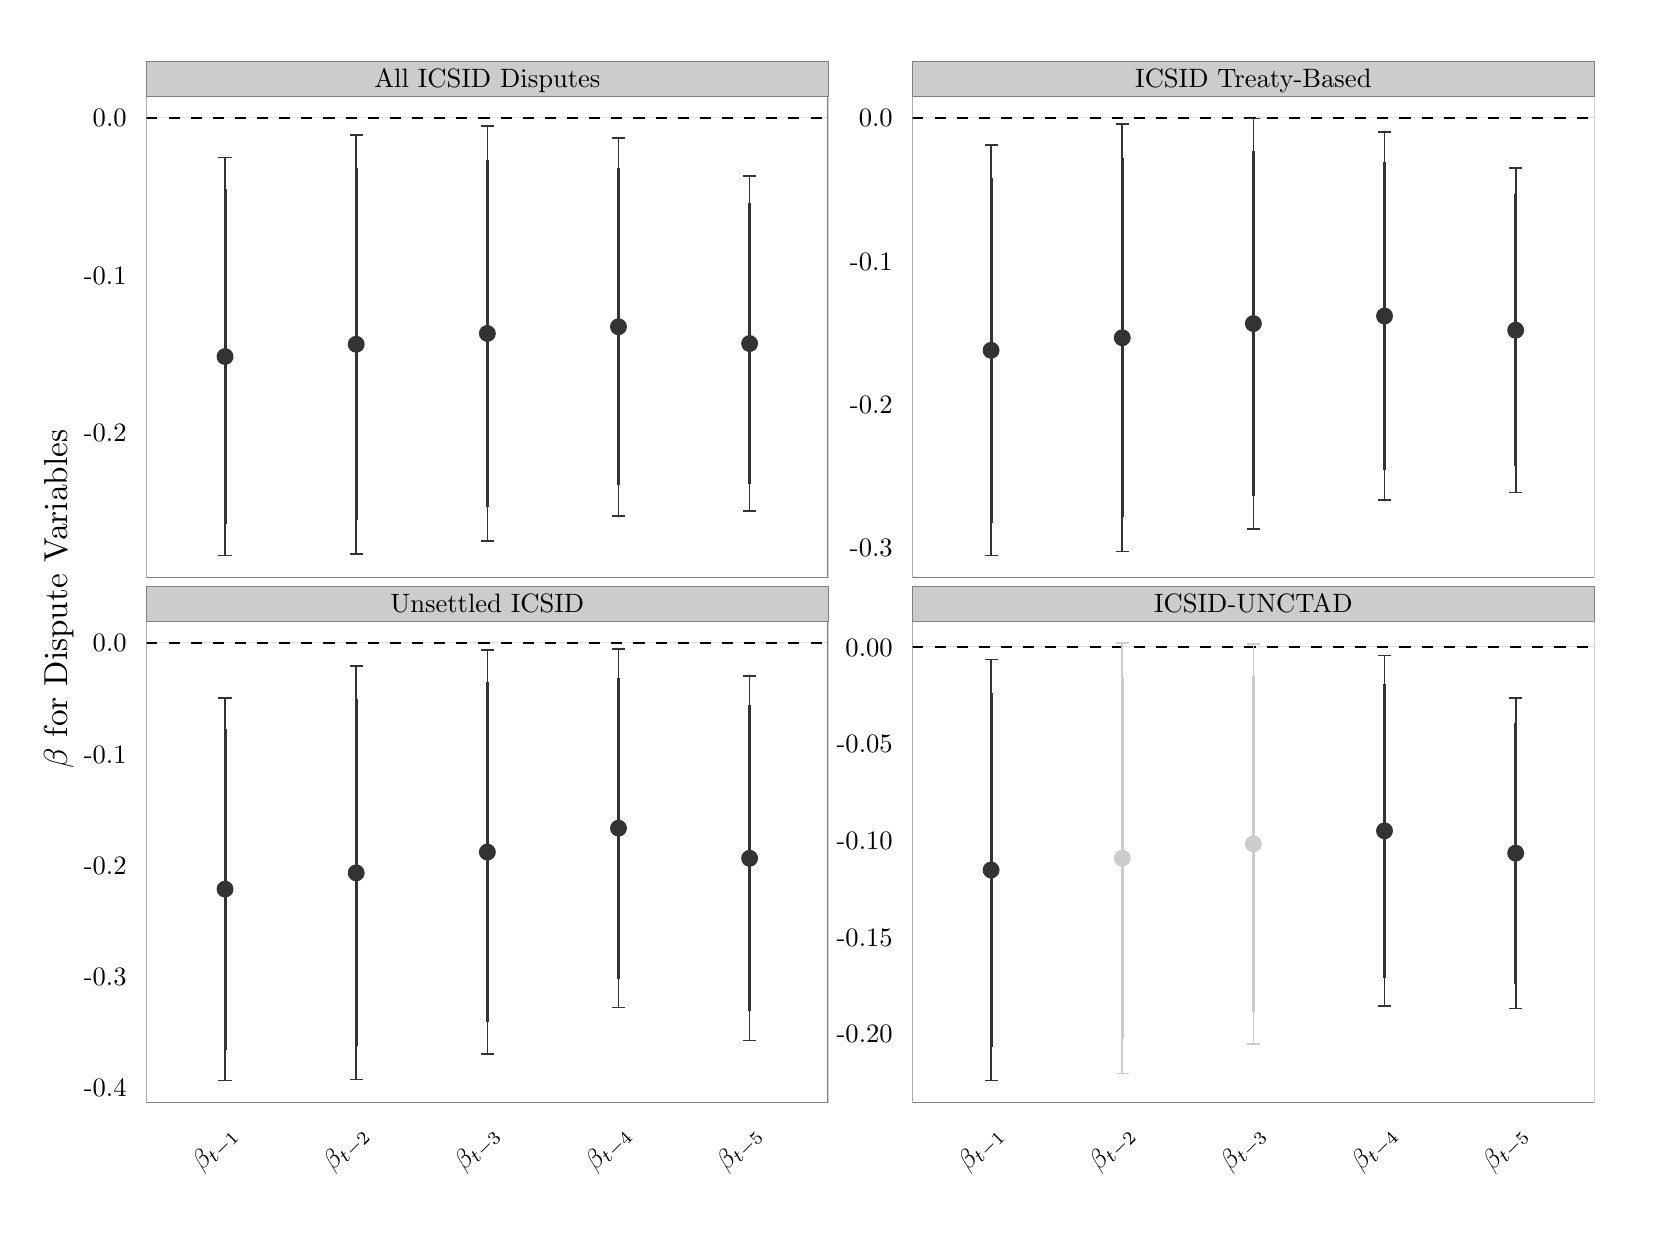
\begin{tikzpicture}[x=1pt,y=1pt]
\definecolor[named]{fillColor}{rgb}{1.00,1.00,1.00}
\path[use as bounding box,fill=fillColor,fill opacity=0.00] (0,0) rectangle (578.16,433.62);
\begin{scope}
\path[clip] (  0.00,  0.00) rectangle (578.16,433.62);
\definecolor[named]{drawColor}{rgb}{1.00,1.00,1.00}
\definecolor[named]{fillColor}{rgb}{1.00,1.00,1.00}

\path[draw=drawColor,line width= 0.6pt,line join=round,line cap=round,fill=fillColor] (  0.00,  0.00) rectangle (578.16,433.62);
\end{scope}
\begin{scope}
\path[clip] ( 42.89,234.93) rectangle (289.31,408.94);
\definecolor[named]{fillColor}{rgb}{1.00,1.00,1.00}

\path[fill=fillColor] ( 42.89,234.93) rectangle (289.31,408.94);
\definecolor[named]{drawColor}{rgb}{0.20,0.20,0.20}
\definecolor[named]{fillColor}{rgb}{0.20,0.20,0.20}

\path[draw=drawColor,draw opacity=0.30,line width= 0.3pt,line join=round,fill=fillColor,fill opacity=0.30] ( 71.32,242.84) -- ( 71.32,386.71);

\path[draw=drawColor,draw opacity=0.30,line width= 0.3pt,line join=round,fill=fillColor,fill opacity=0.30] (118.71,243.49) -- (118.71,394.92);

\path[draw=drawColor,draw opacity=0.30,line width= 0.3pt,line join=round,fill=fillColor,fill opacity=0.30] (166.10,248.24) -- (166.10,398.00);

\path[draw=drawColor,draw opacity=0.30,line width= 0.3pt,line join=round,fill=fillColor,fill opacity=0.30] (213.49,257.24) -- (213.49,393.85);

\path[draw=drawColor,draw opacity=0.30,line width= 0.3pt,line join=round,fill=fillColor,fill opacity=0.30] (260.87,258.85) -- (260.87,380.09);
\definecolor[named]{drawColor}{rgb}{0.20,0.20,0.20}
\definecolor[named]{fillColor}{rgb}{0.20,0.20,0.20}

\path[draw=drawColor,line width= 1.1pt,line join=round,fill=fillColor] ( 71.32,254.41) -- ( 71.32,375.15);

\path[draw=drawColor,line width= 1.1pt,line join=round,fill=fillColor] (118.71,255.66) -- (118.71,382.75);

\path[draw=drawColor,line width= 1.1pt,line join=round,fill=fillColor] (166.10,260.28) -- (166.10,385.96);

\path[draw=drawColor,line width= 1.1pt,line join=round,fill=fillColor] (213.49,268.22) -- (213.49,382.87);

\path[draw=drawColor,line width= 1.1pt,line join=round,fill=fillColor] (260.87,268.60) -- (260.87,370.34);
\definecolor[named]{drawColor}{rgb}{0.00,0.00,0.00}
\definecolor[named]{fillColor}{rgb}{0.00,0.00,0.00}

\path[draw=drawColor,line width= 0.6pt,dash pattern=on 4pt off 4pt ,line join=round,fill=fillColor] ( 42.89,401.03) -- (289.31,401.03);
\definecolor[named]{drawColor}{rgb}{0.20,0.20,0.20}
\definecolor[named]{fillColor}{rgb}{0.20,0.20,0.20}

\path[draw=drawColor,line width= 0.4pt,line join=round,line cap=round,fill=fillColor] ( 71.32,314.78) circle (  2.85);

\path[draw=drawColor,line width= 0.4pt,line join=round,line cap=round,fill=fillColor] (118.71,319.21) circle (  2.85);

\path[draw=drawColor,line width= 0.4pt,line join=round,line cap=round,fill=fillColor] (166.10,323.12) circle (  2.85);

\path[draw=drawColor,line width= 0.4pt,line join=round,line cap=round,fill=fillColor] (213.49,325.55) circle (  2.85);

\path[draw=drawColor,line width= 0.4pt,line join=round,line cap=round,fill=fillColor] (260.87,319.47) circle (  2.85);

\path[draw=drawColor,line width= 0.6pt,line join=round] ( 68.95,386.71) --
	( 73.69,386.71);

\path[draw=drawColor,line width= 0.6pt,line join=round] ( 71.32,386.71) --
	( 71.32,242.84);

\path[draw=drawColor,line width= 0.6pt,line join=round] ( 68.95,242.84) --
	( 73.69,242.84);

\path[draw=drawColor,line width= 0.6pt,line join=round] (116.34,394.92) --
	(121.08,394.92);

\path[draw=drawColor,line width= 0.6pt,line join=round] (118.71,394.92) --
	(118.71,243.49);

\path[draw=drawColor,line width= 0.6pt,line join=round] (116.34,243.49) --
	(121.08,243.49);

\path[draw=drawColor,line width= 0.6pt,line join=round] (163.73,398.00) --
	(168.47,398.00);

\path[draw=drawColor,line width= 0.6pt,line join=round] (166.10,398.00) --
	(166.10,248.24);

\path[draw=drawColor,line width= 0.6pt,line join=round] (163.73,248.24) --
	(168.47,248.24);

\path[draw=drawColor,line width= 0.6pt,line join=round] (211.12,393.85) --
	(215.85,393.85);

\path[draw=drawColor,line width= 0.6pt,line join=round] (213.49,393.85) --
	(213.49,257.24);

\path[draw=drawColor,line width= 0.6pt,line join=round] (211.12,257.24) --
	(215.85,257.24);

\path[draw=drawColor,line width= 0.6pt,line join=round] (258.50,380.09) --
	(263.24,380.09);

\path[draw=drawColor,line width= 0.6pt,line join=round] (260.87,380.09) --
	(260.87,258.85);

\path[draw=drawColor,line width= 0.6pt,line join=round] (258.50,258.85) --
	(263.24,258.85);
\definecolor[named]{drawColor}{rgb}{0.50,0.50,0.50}

\path[draw=drawColor,line width= 0.6pt,line join=round,line cap=round] ( 42.89,234.93) rectangle (289.31,408.94);
\end{scope}
\begin{scope}
\path[clip] (319.69,234.93) rectangle (566.12,408.94);
\definecolor[named]{fillColor}{rgb}{1.00,1.00,1.00}

\path[fill=fillColor] (319.69,234.93) rectangle (566.12,408.94);
\definecolor[named]{drawColor}{rgb}{0.20,0.20,0.20}
\definecolor[named]{fillColor}{rgb}{0.20,0.20,0.20}

\path[draw=drawColor,draw opacity=0.30,line width= 0.3pt,line join=round,fill=fillColor,fill opacity=0.30] (348.13,242.84) -- (348.13,391.24);

\path[draw=drawColor,draw opacity=0.30,line width= 0.3pt,line join=round,fill=fillColor,fill opacity=0.30] (395.52,244.37) -- (395.52,398.76);

\path[draw=drawColor,draw opacity=0.30,line width= 0.3pt,line join=round,fill=fillColor,fill opacity=0.30] (442.90,252.56) -- (442.90,400.82);

\path[draw=drawColor,draw opacity=0.30,line width= 0.3pt,line join=round,fill=fillColor,fill opacity=0.30] (490.29,262.94) -- (490.29,395.90);

\path[draw=drawColor,draw opacity=0.30,line width= 0.3pt,line join=round,fill=fillColor,fill opacity=0.30] (537.68,265.68) -- (537.68,382.87);
\definecolor[named]{drawColor}{rgb}{0.20,0.20,0.20}
\definecolor[named]{fillColor}{rgb}{0.20,0.20,0.20}

\path[draw=drawColor,line width= 1.1pt,line join=round,fill=fillColor] (348.13,254.77) -- (348.13,379.31);

\path[draw=drawColor,line width= 1.1pt,line join=round,fill=fillColor] (395.52,256.78) -- (395.52,386.35);

\path[draw=drawColor,line width= 1.1pt,line join=round,fill=fillColor] (442.90,264.48) -- (442.90,388.90);

\path[draw=drawColor,line width= 1.1pt,line join=round,fill=fillColor] (490.29,273.63) -- (490.29,385.22);

\path[draw=drawColor,line width= 1.1pt,line join=round,fill=fillColor] (537.68,275.10) -- (537.68,373.45);
\definecolor[named]{drawColor}{rgb}{0.00,0.00,0.00}
\definecolor[named]{fillColor}{rgb}{0.00,0.00,0.00}

\path[draw=drawColor,line width= 0.6pt,dash pattern=on 4pt off 4pt ,line join=round,fill=fillColor] (319.69,401.03) -- (566.12,401.03);
\definecolor[named]{drawColor}{rgb}{0.20,0.20,0.20}
\definecolor[named]{fillColor}{rgb}{0.20,0.20,0.20}

\path[draw=drawColor,line width= 0.4pt,line join=round,line cap=round,fill=fillColor] (348.13,317.04) circle (  2.85);

\path[draw=drawColor,line width= 0.4pt,line join=round,line cap=round,fill=fillColor] (395.52,321.57) circle (  2.85);

\path[draw=drawColor,line width= 0.4pt,line join=round,line cap=round,fill=fillColor] (442.90,326.69) circle (  2.85);

\path[draw=drawColor,line width= 0.4pt,line join=round,line cap=round,fill=fillColor] (490.29,329.42) circle (  2.85);

\path[draw=drawColor,line width= 0.4pt,line join=round,line cap=round,fill=fillColor] (537.68,324.28) circle (  2.85);

\path[draw=drawColor,line width= 0.6pt,line join=round] (345.76,391.24) --
	(350.50,391.24);

\path[draw=drawColor,line width= 0.6pt,line join=round] (348.13,391.24) --
	(348.13,242.84);

\path[draw=drawColor,line width= 0.6pt,line join=round] (345.76,242.84) --
	(350.50,242.84);

\path[draw=drawColor,line width= 0.6pt,line join=round] (393.15,398.76) --
	(397.88,398.76);

\path[draw=drawColor,line width= 0.6pt,line join=round] (395.52,398.76) --
	(395.52,244.37);

\path[draw=drawColor,line width= 0.6pt,line join=round] (393.15,244.37) --
	(397.88,244.37);

\path[draw=drawColor,line width= 0.6pt,line join=round] (440.53,400.82) --
	(445.27,400.82);

\path[draw=drawColor,line width= 0.6pt,line join=round] (442.90,400.82) --
	(442.90,252.56);

\path[draw=drawColor,line width= 0.6pt,line join=round] (440.53,252.56) --
	(445.27,252.56);

\path[draw=drawColor,line width= 0.6pt,line join=round] (487.92,395.90) --
	(492.66,395.90);

\path[draw=drawColor,line width= 0.6pt,line join=round] (490.29,395.90) --
	(490.29,262.94);

\path[draw=drawColor,line width= 0.6pt,line join=round] (487.92,262.94) --
	(492.66,262.94);

\path[draw=drawColor,line width= 0.6pt,line join=round] (535.31,382.87) --
	(540.05,382.87);

\path[draw=drawColor,line width= 0.6pt,line join=round] (537.68,382.87) --
	(537.68,265.68);

\path[draw=drawColor,line width= 0.6pt,line join=round] (535.31,265.68) --
	(540.05,265.68);
\definecolor[named]{drawColor}{rgb}{0.50,0.50,0.50}

\path[draw=drawColor,line width= 0.6pt,line join=round,line cap=round] (319.69,234.93) rectangle (566.12,408.94);
\end{scope}
\begin{scope}
\path[clip] ( 42.89, 45.28) rectangle (289.31,219.29);
\definecolor[named]{fillColor}{rgb}{1.00,1.00,1.00}

\path[fill=fillColor] ( 42.89, 45.28) rectangle (289.31,219.29);
\definecolor[named]{drawColor}{rgb}{0.20,0.20,0.20}
\definecolor[named]{fillColor}{rgb}{0.20,0.20,0.20}

\path[draw=drawColor,draw opacity=0.30,line width= 0.3pt,line join=round,fill=fillColor,fill opacity=0.30] ( 71.32, 53.19) -- ( 71.32,191.48);

\path[draw=drawColor,draw opacity=0.30,line width= 0.3pt,line join=round,fill=fillColor,fill opacity=0.30] (118.71, 53.53) -- (118.71,202.87);

\path[draw=drawColor,draw opacity=0.30,line width= 0.3pt,line join=round,fill=fillColor,fill opacity=0.30] (166.10, 62.72) -- (166.10,208.73);

\path[draw=drawColor,draw opacity=0.30,line width= 0.3pt,line join=round,fill=fillColor,fill opacity=0.30] (213.49, 79.60) -- (213.49,209.12);

\path[draw=drawColor,draw opacity=0.30,line width= 0.3pt,line join=round,fill=fillColor,fill opacity=0.30] (260.87, 67.60) -- (260.87,199.33);
\definecolor[named]{drawColor}{rgb}{0.20,0.20,0.20}
\definecolor[named]{fillColor}{rgb}{0.20,0.20,0.20}

\path[draw=drawColor,line width= 1.1pt,line join=round,fill=fillColor] ( 71.32, 64.30) -- ( 71.32,180.37);

\path[draw=drawColor,line width= 1.1pt,line join=round,fill=fillColor] (118.71, 65.53) -- (118.71,190.86);

\path[draw=drawColor,line width= 1.1pt,line join=round,fill=fillColor] (166.10, 74.45) -- (166.10,197.00);

\path[draw=drawColor,line width= 1.1pt,line join=round,fill=fillColor] (213.49, 90.01) -- (213.49,198.71);

\path[draw=drawColor,line width= 1.1pt,line join=round,fill=fillColor] (260.87, 78.19) -- (260.87,188.74);
\definecolor[named]{drawColor}{rgb}{0.00,0.00,0.00}
\definecolor[named]{fillColor}{rgb}{0.00,0.00,0.00}

\path[draw=drawColor,line width= 0.6pt,dash pattern=on 4pt off 4pt ,line join=round,fill=fillColor] ( 42.89,211.38) -- (289.31,211.38);
\definecolor[named]{drawColor}{rgb}{0.20,0.20,0.20}
\definecolor[named]{fillColor}{rgb}{0.20,0.20,0.20}

\path[draw=drawColor,line width= 0.4pt,line join=round,line cap=round,fill=fillColor] ( 71.32,122.33) circle (  2.85);

\path[draw=drawColor,line width= 0.4pt,line join=round,line cap=round,fill=fillColor] (118.71,128.20) circle (  2.85);

\path[draw=drawColor,line width= 0.4pt,line join=round,line cap=round,fill=fillColor] (166.10,135.72) circle (  2.85);

\path[draw=drawColor,line width= 0.4pt,line join=round,line cap=round,fill=fillColor] (213.49,144.36) circle (  2.85);

\path[draw=drawColor,line width= 0.4pt,line join=round,line cap=round,fill=fillColor] (260.87,133.47) circle (  2.85);

\path[draw=drawColor,line width= 0.6pt,line join=round] ( 68.95,191.48) --
	( 73.69,191.48);

\path[draw=drawColor,line width= 0.6pt,line join=round] ( 71.32,191.48) --
	( 71.32, 53.19);

\path[draw=drawColor,line width= 0.6pt,line join=round] ( 68.95, 53.19) --
	( 73.69, 53.19);

\path[draw=drawColor,line width= 0.6pt,line join=round] (116.34,202.87) --
	(121.08,202.87);

\path[draw=drawColor,line width= 0.6pt,line join=round] (118.71,202.87) --
	(118.71, 53.53);

\path[draw=drawColor,line width= 0.6pt,line join=round] (116.34, 53.53) --
	(121.08, 53.53);

\path[draw=drawColor,line width= 0.6pt,line join=round] (163.73,208.73) --
	(168.47,208.73);

\path[draw=drawColor,line width= 0.6pt,line join=round] (166.10,208.73) --
	(166.10, 62.72);

\path[draw=drawColor,line width= 0.6pt,line join=round] (163.73, 62.72) --
	(168.47, 62.72);

\path[draw=drawColor,line width= 0.6pt,line join=round] (211.12,209.12) --
	(215.85,209.12);

\path[draw=drawColor,line width= 0.6pt,line join=round] (213.49,209.12) --
	(213.49, 79.60);

\path[draw=drawColor,line width= 0.6pt,line join=round] (211.12, 79.60) --
	(215.85, 79.60);

\path[draw=drawColor,line width= 0.6pt,line join=round] (258.50,199.33) --
	(263.24,199.33);

\path[draw=drawColor,line width= 0.6pt,line join=round] (260.87,199.33) --
	(260.87, 67.60);

\path[draw=drawColor,line width= 0.6pt,line join=round] (258.50, 67.60) --
	(263.24, 67.60);
\definecolor[named]{drawColor}{rgb}{0.50,0.50,0.50}

\path[draw=drawColor,line width= 0.6pt,line join=round,line cap=round] ( 42.89, 45.28) rectangle (289.31,219.29);
\end{scope}
\begin{scope}
\path[clip] (319.69, 45.28) rectangle (566.12,219.29);
\definecolor[named]{fillColor}{rgb}{1.00,1.00,1.00}

\path[fill=fillColor] (319.69, 45.28) rectangle (566.12,219.29);
\definecolor[named]{drawColor}{rgb}{0.20,0.20,0.20}
\definecolor[named]{fillColor}{rgb}{0.20,0.20,0.20}

\path[draw=drawColor,draw opacity=0.30,line width= 0.3pt,line join=round,fill=fillColor,fill opacity=0.30] (348.13, 53.19) -- (348.13,205.30);
\definecolor[named]{drawColor}{rgb}{0.80,0.80,0.80}
\definecolor[named]{fillColor}{rgb}{0.80,0.80,0.80}

\path[draw=drawColor,draw opacity=0.30,line width= 0.3pt,line join=round,fill=fillColor,fill opacity=0.30] (395.52, 55.67) -- (395.52,211.38);

\path[draw=drawColor,draw opacity=0.30,line width= 0.3pt,line join=round,fill=fillColor,fill opacity=0.30] (442.90, 66.46) -- (442.90,210.94);
\definecolor[named]{drawColor}{rgb}{0.20,0.20,0.20}
\definecolor[named]{fillColor}{rgb}{0.20,0.20,0.20}

\path[draw=drawColor,draw opacity=0.30,line width= 0.3pt,line join=round,fill=fillColor,fill opacity=0.30] (490.29, 79.99) -- (490.29,206.79);

\path[draw=drawColor,draw opacity=0.30,line width= 0.3pt,line join=round,fill=fillColor,fill opacity=0.30] (537.68, 79.19) -- (537.68,191.47);
\definecolor[named]{drawColor}{rgb}{0.20,0.20,0.20}
\definecolor[named]{fillColor}{rgb}{0.20,0.20,0.20}

\path[draw=drawColor,line width= 1.1pt,line join=round,fill=fillColor] (348.13, 65.41) -- (348.13,193.07);
\definecolor[named]{drawColor}{rgb}{0.80,0.80,0.80}
\definecolor[named]{fillColor}{rgb}{0.80,0.80,0.80}

\path[draw=drawColor,line width= 1.1pt,line join=round,fill=fillColor] (395.52, 68.19) -- (395.52,198.86);

\path[draw=drawColor,line width= 1.1pt,line join=round,fill=fillColor] (442.90, 78.07) -- (442.90,199.33);
\definecolor[named]{drawColor}{rgb}{0.20,0.20,0.20}
\definecolor[named]{fillColor}{rgb}{0.20,0.20,0.20}

\path[draw=drawColor,line width= 1.1pt,line join=round,fill=fillColor] (490.29, 90.18) -- (490.29,196.60);

\path[draw=drawColor,line width= 1.1pt,line join=round,fill=fillColor] (537.68, 88.22) -- (537.68,182.45);
\definecolor[named]{drawColor}{rgb}{0.00,0.00,0.00}
\definecolor[named]{fillColor}{rgb}{0.00,0.00,0.00}

\path[draw=drawColor,line width= 0.6pt,dash pattern=on 4pt off 4pt ,line join=round,fill=fillColor] (319.69,209.87) -- (566.12,209.87);
\definecolor[named]{drawColor}{rgb}{0.20,0.20,0.20}
\definecolor[named]{fillColor}{rgb}{0.20,0.20,0.20}

\path[draw=drawColor,line width= 0.4pt,line join=round,line cap=round,fill=fillColor] (348.13,129.24) circle (  2.85);
\definecolor[named]{drawColor}{rgb}{0.80,0.80,0.80}
\definecolor[named]{fillColor}{rgb}{0.80,0.80,0.80}

\path[draw=drawColor,line width= 0.4pt,line join=round,line cap=round,fill=fillColor] (395.52,133.52) circle (  2.85);

\path[draw=drawColor,line width= 0.4pt,line join=round,line cap=round,fill=fillColor] (442.90,138.70) circle (  2.85);
\definecolor[named]{drawColor}{rgb}{0.20,0.20,0.20}
\definecolor[named]{fillColor}{rgb}{0.20,0.20,0.20}

\path[draw=drawColor,line width= 0.4pt,line join=round,line cap=round,fill=fillColor] (490.29,143.39) circle (  2.85);

\path[draw=drawColor,line width= 0.4pt,line join=round,line cap=round,fill=fillColor] (537.68,135.33) circle (  2.85);

\path[draw=drawColor,line width= 0.6pt,line join=round] (345.76,205.30) --
	(350.50,205.30);

\path[draw=drawColor,line width= 0.6pt,line join=round] (348.13,205.30) --
	(348.13, 53.19);

\path[draw=drawColor,line width= 0.6pt,line join=round] (345.76, 53.19) --
	(350.50, 53.19);
\definecolor[named]{drawColor}{rgb}{0.80,0.80,0.80}

\path[draw=drawColor,line width= 0.6pt,line join=round] (393.15,211.38) --
	(397.88,211.38);

\path[draw=drawColor,line width= 0.6pt,line join=round] (395.52,211.38) --
	(395.52, 55.67);

\path[draw=drawColor,line width= 0.6pt,line join=round] (393.15, 55.67) --
	(397.88, 55.67);

\path[draw=drawColor,line width= 0.6pt,line join=round] (440.53,210.94) --
	(445.27,210.94);

\path[draw=drawColor,line width= 0.6pt,line join=round] (442.90,210.94) --
	(442.90, 66.46);

\path[draw=drawColor,line width= 0.6pt,line join=round] (440.53, 66.46) --
	(445.27, 66.46);
\definecolor[named]{drawColor}{rgb}{0.20,0.20,0.20}

\path[draw=drawColor,line width= 0.6pt,line join=round] (487.92,206.79) --
	(492.66,206.79);

\path[draw=drawColor,line width= 0.6pt,line join=round] (490.29,206.79) --
	(490.29, 79.99);

\path[draw=drawColor,line width= 0.6pt,line join=round] (487.92, 79.99) --
	(492.66, 79.99);

\path[draw=drawColor,line width= 0.6pt,line join=round] (535.31,191.47) --
	(540.05,191.47);

\path[draw=drawColor,line width= 0.6pt,line join=round] (537.68,191.47) --
	(537.68, 79.19);

\path[draw=drawColor,line width= 0.6pt,line join=round] (535.31, 79.19) --
	(540.05, 79.19);
\definecolor[named]{drawColor}{rgb}{0.50,0.50,0.50}

\path[draw=drawColor,line width= 0.6pt,line join=round,line cap=round] (319.69, 45.28) rectangle (566.12,219.29);
\end{scope}
\begin{scope}
\path[clip] (  0.00,  0.00) rectangle (578.16,433.62);
\definecolor[named]{drawColor}{rgb}{0.50,0.50,0.50}
\definecolor[named]{fillColor}{rgb}{0.80,0.80,0.80}

\path[draw=drawColor,line width= 0.2pt,line join=round,line cap=round,fill=fillColor] ( 42.89,408.94) rectangle (289.31,421.57);
\definecolor[named]{drawColor}{rgb}{0.00,0.00,0.00}

\node[text=drawColor,anchor=base,inner sep=0pt, outer sep=0pt, scale=  0.96] at (166.10,411.95) {All ICSID Disputes};
\end{scope}
\begin{scope}
\path[clip] (  0.00,  0.00) rectangle (578.16,433.62);
\definecolor[named]{drawColor}{rgb}{0.50,0.50,0.50}
\definecolor[named]{fillColor}{rgb}{0.80,0.80,0.80}

\path[draw=drawColor,line width= 0.2pt,line join=round,line cap=round,fill=fillColor] (319.69,408.94) rectangle (566.12,421.57);
\definecolor[named]{drawColor}{rgb}{0.00,0.00,0.00}

\node[text=drawColor,anchor=base,inner sep=0pt, outer sep=0pt, scale=  0.96] at (442.90,411.95) {ICSID Treaty-Based};
\end{scope}
\begin{scope}
\path[clip] (  0.00,  0.00) rectangle (578.16,433.62);
\definecolor[named]{drawColor}{rgb}{0.50,0.50,0.50}
\definecolor[named]{fillColor}{rgb}{0.80,0.80,0.80}

\path[draw=drawColor,line width= 0.2pt,line join=round,line cap=round,fill=fillColor] ( 42.89,219.29) rectangle (289.31,231.92);
\definecolor[named]{drawColor}{rgb}{0.00,0.00,0.00}

\node[text=drawColor,anchor=base,inner sep=0pt, outer sep=0pt, scale=  0.96] at (166.10,222.30) {Unsettled ICSID};
\end{scope}
\begin{scope}
\path[clip] (  0.00,  0.00) rectangle (578.16,433.62);
\definecolor[named]{drawColor}{rgb}{0.50,0.50,0.50}
\definecolor[named]{fillColor}{rgb}{0.80,0.80,0.80}

\path[draw=drawColor,line width= 0.2pt,line join=round,line cap=round,fill=fillColor] (319.69,219.29) rectangle (566.12,231.92);
\definecolor[named]{drawColor}{rgb}{0.00,0.00,0.00}

\node[text=drawColor,anchor=base,inner sep=0pt, outer sep=0pt, scale=  0.96] at (442.90,222.30) {ICSID-UNCTAD};
\end{scope}
\begin{scope}
\path[clip] (  0.00,  0.00) rectangle (578.16,433.62);
\definecolor[named]{drawColor}{rgb}{0.00,0.00,0.00}

\node[text=drawColor,anchor=base east,inner sep=0pt, outer sep=0pt, scale=  0.96] at ( 35.77,284.06) {-0.2};

\node[text=drawColor,anchor=base east,inner sep=0pt, outer sep=0pt, scale=  0.96] at ( 35.77,340.89) {-0.1};

\node[text=drawColor,anchor=base east,inner sep=0pt, outer sep=0pt, scale=  0.96] at ( 35.77,397.73) {0.0};
\end{scope}
\begin{scope}
\path[clip] (  0.00,  0.00) rectangle (578.16,433.62);
\definecolor[named]{drawColor}{rgb}{0.00,0.00,0.00}

\node[text=drawColor,anchor=base east,inner sep=0pt, outer sep=0pt, scale=  0.96] at (312.58,242.61) {-0.3};

\node[text=drawColor,anchor=base east,inner sep=0pt, outer sep=0pt, scale=  0.96] at (312.58,294.31) {-0.2};

\node[text=drawColor,anchor=base east,inner sep=0pt, outer sep=0pt, scale=  0.96] at (312.58,346.02) {-0.1};

\node[text=drawColor,anchor=base east,inner sep=0pt, outer sep=0pt, scale=  0.96] at (312.58,397.73) {0.0};
\end{scope}
\begin{scope}
\path[clip] (  0.00,  0.00) rectangle (578.16,433.62);
\definecolor[named]{drawColor}{rgb}{0.00,0.00,0.00}

\node[text=drawColor,anchor=base east,inner sep=0pt, outer sep=0pt, scale=  0.96] at ( 35.77, 47.23) {-0.4};

\node[text=drawColor,anchor=base east,inner sep=0pt, outer sep=0pt, scale=  0.96] at ( 35.77, 87.44) {-0.3};

\node[text=drawColor,anchor=base east,inner sep=0pt, outer sep=0pt, scale=  0.96] at ( 35.77,127.65) {-0.2};

\node[text=drawColor,anchor=base east,inner sep=0pt, outer sep=0pt, scale=  0.96] at ( 35.77,167.86) {-0.1};

\node[text=drawColor,anchor=base east,inner sep=0pt, outer sep=0pt, scale=  0.96] at ( 35.77,208.07) {0.0};
\end{scope}
\begin{scope}
\path[clip] (  0.00,  0.00) rectangle (578.16,433.62);
\definecolor[named]{drawColor}{rgb}{0.00,0.00,0.00}

\node[text=drawColor,anchor=base east,inner sep=0pt, outer sep=0pt, scale=  0.96] at (312.58, 66.83) {-0.20};

\node[text=drawColor,anchor=base east,inner sep=0pt, outer sep=0pt, scale=  0.96] at (312.58,101.76) {-0.15};

\node[text=drawColor,anchor=base east,inner sep=0pt, outer sep=0pt, scale=  0.96] at (312.58,136.69) {-0.10};

\node[text=drawColor,anchor=base east,inner sep=0pt, outer sep=0pt, scale=  0.96] at (312.58,171.63) {-0.05};

\node[text=drawColor,anchor=base east,inner sep=0pt, outer sep=0pt, scale=  0.96] at (312.58,206.56) {0.00};
\end{scope}
\begin{scope}
\path[clip] (  0.00,  0.00) rectangle (578.16,433.62);
\definecolor[named]{drawColor}{rgb}{0.00,0.00,0.00}

\node[text=drawColor,rotate= 45.00,anchor=base east,inner sep=0pt, outer sep=0pt, scale=  0.96] at ( 75.99, 33.49) {$\beta_{t-1}$};

\node[text=drawColor,rotate= 45.00,anchor=base east,inner sep=0pt, outer sep=0pt, scale=  0.96] at (123.38, 33.49) {$\beta_{t-2}$};

\node[text=drawColor,rotate= 45.00,anchor=base east,inner sep=0pt, outer sep=0pt, scale=  0.96] at (170.77, 33.49) {$\beta_{t-3}$};

\node[text=drawColor,rotate= 45.00,anchor=base east,inner sep=0pt, outer sep=0pt, scale=  0.96] at (218.16, 33.49) {$\beta_{t-4}$};

\node[text=drawColor,rotate= 45.00,anchor=base east,inner sep=0pt, outer sep=0pt, scale=  0.96] at (265.55, 33.49) {$\beta_{t-5}$};
\end{scope}
\begin{scope}
\path[clip] (  0.00,  0.00) rectangle (578.16,433.62);
\definecolor[named]{drawColor}{rgb}{0.00,0.00,0.00}

\node[text=drawColor,rotate= 45.00,anchor=base east,inner sep=0pt, outer sep=0pt, scale=  0.96] at (352.80, 33.49) {$\beta_{t-1}$};

\node[text=drawColor,rotate= 45.00,anchor=base east,inner sep=0pt, outer sep=0pt, scale=  0.96] at (400.19, 33.49) {$\beta_{t-2}$};

\node[text=drawColor,rotate= 45.00,anchor=base east,inner sep=0pt, outer sep=0pt, scale=  0.96] at (447.58, 33.49) {$\beta_{t-3}$};

\node[text=drawColor,rotate= 45.00,anchor=base east,inner sep=0pt, outer sep=0pt, scale=  0.96] at (494.97, 33.49) {$\beta_{t-4}$};

\node[text=drawColor,rotate= 45.00,anchor=base east,inner sep=0pt, outer sep=0pt, scale=  0.96] at (542.36, 33.49) {$\beta_{t-5}$};
\end{scope}
\begin{scope}
\path[clip] (  0.00,  0.00) rectangle (578.16,433.62);
\definecolor[named]{drawColor}{rgb}{0.00,0.00,0.00}

\node[text=drawColor,rotate= 90.00,anchor=base,inner sep=0pt, outer sep=0pt, scale=  1.20] at ( 14.29,227.11) {$\beta$ for Dispute Variables};
\end{scope}
\end{tikzpicture}
